\documentclass[journal,comsoc]{IEEEtran}
\usepackage{graphicx}
\usepackage{lipsum} % For generating placeholder text
\usepackage{cite}

\usepackage[numbers]{natbib}
\usepackage{adjustbox}
\usepackage{caption}
\usepackage{url}
\usepackage{comment}
\usepackage[labelformat=simple]{subcaption}
\renewcommand\thesubfigure{\alph{subfigure}}
\DeclareCaptionLabelFormat{subcaptionlabel}{\normalfont(\textbf{#2}\normalfont)}
%captionsetup[subfigure]{labelformat=subcaptionlabel,justification=centering}

\usepackage[utf8]{inputenc}
\usepackage{amsmath}
\usepackage{amssymb}
\usepackage{booktabs}
\usepackage{url}
\usepackage{hyperref}
\usepackage{graphicx}
\usepackage{tikz}
\usepackage{xcolor}
\usetikzlibrary{shapes.geometric, arrows, positioning, fit, backgrounds, calc}

\title{INVESTRA: A Modular Machine Learning Pipeline for Gold
Price Forecasting and Investment Decision Support}

\author{
\IEEEauthorblockN{Rakibul Islam Asif, Md Emon Biswas, Md Rafiu Islam, Md Siyam Shanto, Md Mehedi Hasan Rafi}\\
\IEEEauthorblockA{
Department of Computer Science and Engineering\\
Bangladesh University Of Business and Technology\\
Dhaka, Bangladesh
}
}

\begin{document}
\maketitle

%------------------------------------------------------------------
\begin{abstract}
Gold price forecasting remains a fundamental yet challenging problem in computational finance, owing to the nonlinear, non-stationary, and highly volatile nature of commodity markets. This paper introduces INVESTRA, a modular end-to-end framework that unifies data ingestion, feature engineering, multi-model forecasting, and investor-facing decision support under a single reproducible pipeline. Three distinct forecasting paradigms are integrated and evaluated: XGBoost, a gradient-boosted tree ensemble; Long Short-Term Memory (LSTM), a deep recurrent architecture; and Prophet, a decomposable additive time-series model. Beyond point prediction, INVESTRA incorporates a rule-based recommendation layer that translates numerical forecasts and uncertainty proxies into actionable Buy, Hold, or Sell signals. The system exposes a RESTful FastAPI service and an interactive Streamlit dashboard for practical deployment. Experiments conducted on historical gold OHLCV data demonstrate that Prophet achieves the best error-based performance (MAE = 399.94, RMSE = 698.30, MAPE = 12.87\%, R\textsuperscript{2} = 0.255), while XGBoost attains the highest Directional Accuracy of 77.77\%. These complementary strengths highlight that no single model dominates all investor objectives, motivating the multi-metric, multi-model design of INVESTRA.
\end{abstract}

\begin{IEEEkeywords}
Gold Price Forecasting, Time-Series Prediction, XGBoost, LSTM, Prophet, Decision Support System, FastAPI, Streamlit, Feature Engineering, Financial Machine Learning
\end{IEEEkeywords}

%------------------------------------------------------------------
\section{Introduction}
\label{sec:introduction}
\IEEEPARstart{T}{he} Gold has historically functioned as a safe-haven asset, store of value, and inflation hedge across global financial markets \cite{bollerslev1986generalized}. Its price is driven by a complex interaction of macroeconomic forces including interest rates, currency fluctuations, geopolitical events, and investor sentiment, making it one of the most studied yet difficult-to-predict financial time series \cite{friedman2001greedy}. Even small improvements in forecast accuracy can translate into significant portfolio gains, motivating continued research into advanced prediction methods.

Classical econometric methods such as ARIMA \cite{ashish2017attention} and GARCH \cite{hochreiter1997long} have been widely applied to commodity price forecasting. However, they rely on stationarity assumptions and struggle to capture the complex nonlinear dynamics of modern markets. The advent of machine learning and deep learning has opened new avenues for financial forecasting, with gradient-boosted trees \cite{taylor2018forecasting} and recurrent neural networks \cite{chen2016xgboost} demonstrating strong empirical performance on sequential financial data.

Despite these advances, most existing works evaluate models in isolation, optimizing for a single metric such as mean squared error. Real investor decisions require a broader view: a trader cares not only about how close the predicted price is to the actual value, but whether the predicted direction of movement is correct. Furthermore, few systems bridge the gap between research-grade forecasting and production-ready interfaces that non-technical investors can use.

INVESTRA addresses these gaps through four core contributions:
\begin{enumerate}
    \item A fully modular and reproducible gold price forecasting pipeline covering data ingestion, feature engineering, model training, serialization, and deployment.
    \item A unified comparative evaluation of three complementary forecasting paradigms—XGBoost, LSTM, and Prophet—under identical data splits and evaluation protocols.
    \item A rule-based recommendation engine that converts predicted price movements and confidence proxies into Buy/Hold/Sell signals for investor-facing interpretation.
    \item Production-ready deployment via a FastAPI REST service and a Streamlit interactive dashboard, enabling real-time usage by end-users without programming expertise.
\end{enumerate}

The remainder of this paper is organized as follows. Section II reviews related work. Section III details the methodology and system architecture. Section IV describes the experimental setup. Section V presents and analyzes results. Section VI provides discussion, and Section VII concludes with future directions.

%------------------------------------------------------------------
\section{Related Work}

\subsection{Statistical and Econometric Approaches}
Early gold price forecasting relied on statistical models. Autoregressive Integrated Moving Average (ARIMA) models \cite{faff1999oi} capture linear autocorrelation structures in stationary time series. Generalized Autoregressive Conditional Heteroskedasticity (GARCH) models \cite{box1976analysis} extend this to volatility clustering, which is a common feature of commodity markets. While interpretable, these models assume linearity and often underperform in rapidly shifting market regimes.

\subsection{Machine Learning Methods}
Gradient-boosted decision trees, particularly XGBoost \cite{lecun2015deep}, have demonstrated competitive performance on tabular financial data. By training ensembles of shallow trees with gradient descent, XGBoost handles nonlinear feature interactions and is robust to outliers. Random forests and Support Vector Machines (SVM) have also been applied to gold price prediction \cite{makridakis2018statistical}, though they often require careful feature engineering and hyperparameter tuning.
Gradient-boosted decision trees, particularly XGBoost \cite{jiang2017deep}, have demonstrated competitive performance on tabular financial data. By training ensembles of shallow trees with gradient descent, XGBoost handles nonlinear feature interactions and is robust to outliers. Random forests and Support Vector Machines (SVM) have also been applied to gold price prediction \cite{tay2001application}, though they often require careful feature engineering and hyperparameter tuning.

\subsection{Deep Learning Approaches}
Long Short-Term Memory (LSTM) networks are widely adopted for sequential financial data. Their gating mechanisms allow the network to selectively retain and forget temporal information over long horizons. Bidirectional LSTMs and attention-augmented variants have further improved performance by enabling both forward and backward temporal context. Convolutional-LSTM hybrids have also been explored for multivariate financial signals \cite{yu2019review}.

\subsection{Decomposable and Hybrid Models}
Prophet offers a different paradigm: an additive model that explicitly decomposes a time series into trend, seasonality, and holiday components. Its interpretability and robustness to missing data make it attractive for financial applications with irregular trading calendars. Hybrid approaches combining statistical decomposition with machine learning residual correction have shown promise \cite{chen2009overview}.

\subsection{Decision Support in Finance}
While forecasting accuracy is critical, translating predictions into actionable signals remains underexplored. Rule-based expert systems and reinforcement learning agents have been proposed for trading signal generation. We contributes to this area with a lightweight, interpretable rule engine that requires no additional training data beyond the forecasting output.

%------------------------------------------------------------------
\section{Methodology}

\subsection{Dataset}
The dataset used in this study is the \textit{Gold Price Dynamics} dataset sourced from Kaggle, comprising daily Open, High, Low, Close, and Volume (OHLCV) records spanning multiple decades. The dataset captures diverse market regimes including bull runs, financial crises, and geopolitical shocks, providing a challenging and representative benchmark for forecasting models. Prior to modeling, the dataset undergoes a rigorous preprocessing pipeline described below.

\subsection{Data Ingestion and Preprocessing}
The ingestion module is designed for robustness across varying data formats. Key steps include:
\begin{itemize}
    \item \textbf{Date Parsing:} Multiple date format handlers (ISO 8601, US-format, and epoch) are tried sequentially to ensure compatibility.
    \item \textbf{Numeric Sanitization:} Market price columns are coerced to float; comma-separated values and currency symbols are stripped.
    \item \textbf{Deduplication:} Duplicate date entries are removed, retaining the most recent record.
    \item \textbf{Missing Value Filtering:} Rows with null values in critical price columns are dropped.
    \item \textbf{Chronological Indexing:} The DataFrame is reindexed by date in ascending order to ensure temporal integrity.
\end{itemize}

\subsection{Feature Engineering}
A rich feature set is constructed to encode temporal patterns for supervised learning models (XGBoost and LSTM):
\begin{itemize}
    \item \textbf{Lag Features:} \texttt{Lag\_1}, \texttt{Lag\_2}, \texttt{Lag\_3} — closing prices at 1, 2, and 3 days prior, encoding short-term momentum.
    \item \textbf{Moving Averages:} \texttt{MA\_7} and \texttt{MA\_30} — 7-day and 30-day rolling means, capturing weekly and monthly trend signals.
    \item \textbf{Volatility Proxy:} \texttt{High $-$ Low} — the daily trading range, serving as a measure of intraday price uncertainty.
    \item \textbf{Return Features:} \texttt{Return\_1} and \texttt{Return\_7} — percentage returns over 1 and 7 days, encoding short- and medium-term momentum.
\end{itemize}
Prophet bypasses this tabular feature set, operating directly on the date-close time series using its internal decomposition.

\subsection{Forecasting Models}

\subsubsection{XGBoost Regressor}
XGBoost \cite{patel2022encoding} is trained on the engineered feature matrix with a chronological 80/20 train-test split. The model employs early stopping on a validation subset to prevent overfitting. Tree depth, learning rate, and regularization parameters are configured for financial time-series data. The serialized model is saved for serving via the FastAPI backend.

\subsubsection{Long Short-Term Memory (LSTM)}
The LSTM model \cite{graves2012long} consumes sequences of normalized price windows. Input features are scaled using MinMaxScaler to the $[0,1]$ range. The network comprises two stacked LSTM layers with dropout regularization ($p = 0.2$) and a dense output layer. Training uses the Adam optimizer with mean squared error loss. Sequences of length 60 days are used as the input window.

\subsubsection{Prophet}
Prophet receives a two-column \texttt{(ds, y)} DataFrame where \texttt{ds} is the date and \texttt{y} is the closing price. It automatically fits trend changepoints, weekly seasonality, and yearly seasonality components. The model also produces prediction intervals, which INVESTRA repurposes as an uncertainty proxy for the recommendation layer.

\subsection{System Architecture}

Figure~\ref{fig:architecture} illustrates the complete system architecture of INVESTRA. The framework is divided into three layers: the \textit{Offline Training Layer}, the \textit{Serving Layer}, and the \textit{Presentation Layer}.

\begin{figure*}[t]
\centering
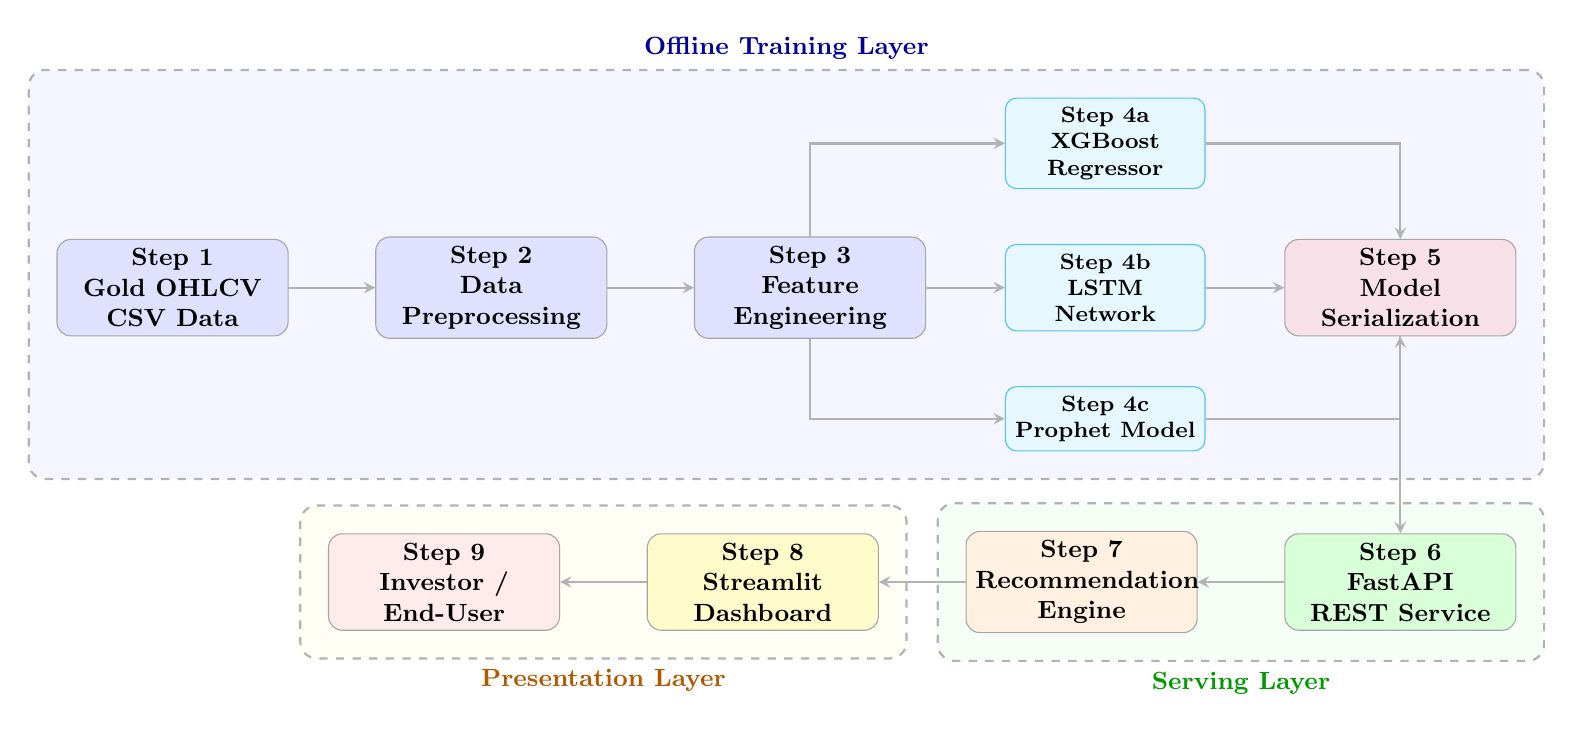
\begin{tikzpicture}[
    node distance=0.8cm and 1.1cm,
    mainbox/.style={rectangle, draw=gray!70, rounded corners=5pt, text centered,
                    font=\small\bfseries, minimum height=1.1cm, text width=2.7cm, fill=white},
    modelbox/.style={rectangle, draw=cyan!70, rounded corners=4pt, text centered,
                    font=\footnotesize\bfseries, minimum height=0.75cm, text width=2.3cm, fill=cyan!10},
    grp/.style={rectangle, draw=gray!60, rounded corners=6pt, dashed, thick, inner sep=10pt},
    arr/.style={->, >=stealth, thick, draw=gray!60}
]

%% ===== ROW 1 (left to right): Offline Training =====
\node[mainbox, fill=blue!12] (csv)  {\textbf{Step 1}\\Gold OHLCV\\CSV Data};
\node[mainbox, fill=blue!12, right=1.1cm of csv]  (pre)  {\textbf{Step 2}\\Data\\Preprocessing};
\node[mainbox, fill=blue!12, right=1.1cm of pre]  (feat) {\textbf{Step 3}\\Feature\\Engineering};

%% Three model nodes (vertical stack, right of feat)
\node[modelbox, above right=0.6cm and 1.0cm of feat] (xgb)  {\textbf{Step 4a}\\XGBoost Regressor};
\node[modelbox, right=1.0cm of feat]                 (lstm) {\textbf{Step 4b}\\LSTM Network};
\node[modelbox, below right=0.6cm and 1.0cm of feat] (prop) {\textbf{Step 4c}\\Prophet Model};

%% Serialization (right of model column)
\node[mainbox, fill=purple!12, right=1.0cm of lstm] (ser) {\textbf{Step 5}\\Model\\Serialization};

%% ===== ROW 2 (right to left): Serving + Presentation =====
\node[mainbox, fill=green!15, below=2.5cm of ser]  (api)  {\textbf{Step 6}\\FastAPI\\REST Service};
\node[mainbox, fill=orange!12, left=1.1cm of api]  (rec)  {\textbf{Step 7}\\Recommendation\\Engine};
\node[mainbox, fill=yellow!20, left=1.1cm of rec]  (dash) {\textbf{Step 8}\\Streamlit\\Dashboard};
\node[mainbox, fill=red!8,     left=1.1cm of dash] (user) {\textbf{Step 9}\\Investor /\\End-User};

%% ===== ARROWS: Row 1 =====
\draw[arr] (csv)        -- (pre);
\draw[arr] (pre)        -- (feat);
\draw[arr] (feat.north) |- (xgb.west);
\draw[arr] (feat)       -- (lstm);
\draw[arr] (feat.south) |- (prop.west);
\draw[arr] (xgb.east)   -| (ser.north);
\draw[arr] (lstm)       -- (ser);
\draw[arr] (prop.east)  -| (ser.south);

%% ===== ARROW: Row 1 to Row 2 =====
\draw[arr] (ser.south) -- (api.north);

%% ===== ARROWS: Row 2 =====
\draw[arr] (api)  -- (rec);
\draw[arr] (rec)  -- (dash);
\draw[arr] (dash) -- (user);

%% ===== GROUP BOXES =====
\begin{scope}[on background layer]
  \node[grp, fill=blue!4,
        fit=(csv)(pre)(feat)(xgb)(lstm)(prop)(ser),
        label={[blue!60!black, font=\small\bfseries]above:Offline Training Layer}] {};
  \node[grp, fill=green!4,
        fit=(api)(rec),
        label={[green!60!black, font=\small\bfseries]below:Serving Layer}] {};
  \node[grp, fill=yellow!4,
        fit=(dash)(user),
        label={[orange!70!black, font=\small\bfseries]below:Presentation Layer}] {};
\end{scope}

\end{tikzpicture}
\caption{System Architecture. }
\label{fig:architecture}
\end{figure*}

\subsection{Deployment Layer}
The FastAPI backend exposes two primary endpoints: \texttt{/predict} for single-step inference given a feature vector, and \texttt{/forecast/latest} for returning a pre-computed daily forecast array. Models are loaded once at startup from serialized artifacts, ensuring low-latency responses. The Streamlit dashboard provides interactive visualizations of historical prices, model predictions, and recommendation signals, requiring no programming knowledge from the end-user.

\subsection{Recommendation Layer}
The recommendation engine applies a rule-based threshold policy on the model outputs. Given the current closing price $P_t$, the predicted next-day price $\hat{P}_{t+1}$, and an uncertainty proxy $\sigma$ (derived from Prophet's prediction interval width), the recommendation signal $R$ is defined as:

\begin{equation}
R = \begin{cases}
\text{BUY}  & \text{if } \hat{P}_{t+1} > P_t + \alpha\,\sigma \\
\text{SELL} & \text{if } \hat{P}_{t+1} < P_t - \alpha\,\sigma \\
\text{HOLD} & \text{otherwise}
\end{cases}
\end{equation}

where $\alpha$ is a sensitivity parameter controlling the signal's conservatism. Figure~\ref{fig:final_decision} shows the resulting Buy/Hold/Sell decision graph over the test period.

\begin{figure}[h]
\centering

\includegraphics[width=\columnwidth]{final_decision_graph.png}
\caption{Final Decision Graph.}

\label{fig:final_decision}
\end{figure}


%------------------------------------------------------------------
\section{Experimental Setup}

\subsection{Dataset Split}
The dataset is partitioned chronologically using a fixed 80/20 train-test ratio to prevent temporal leakage. No shuffling is applied at any stage, ensuring that all models are evaluated strictly on unseen future data. The training set contains earlier historical records, while the test set consists of the most recent 20\% of trading days.

\subsection{Model Configuration}
\begin{itemize}
    \item \textbf{XGBoost:} 500 estimators, max depth = 6, learning rate = 0.05, early stopping rounds = 50 on a 10\% validation split drawn from the training set.
    \item \textbf{LSTM:} 2 stacked LSTM layers (128 and 64 units), dropout = 0.2, sequence length = 60, batch size = 32, 50 epochs with early stopping on validation loss.
    \item \textbf{Prophet:} Default changepoint prior scale, weekly and yearly seasonality enabled, multiplicative seasonality mode.
\end{itemize}

\subsection{Evaluation Protocol}
All models are evaluated on the identical held-out test set using five metrics: MAE, RMSE, R\textsuperscript{2}, MAPE, and Directional Accuracy (DA). This protocol ensures a fair and reproducible comparison across model families with different underlying assumptions.

%------------------------------------------------------------------
\section{Experimental Results}

\subsection{Evaluation Metrics}
Model performance is assessed using the following metrics:
\begin{equation}
    \text{MAE} = \frac{1}{N} \sum_{i=1}^{N} |y_i - \hat{y}_i|
\end{equation}
\begin{equation}
    \text{RMSE} = \sqrt{\frac{1}{N} \sum_{i=1}^{N} (y_i - \hat{y}_i)^2}
\end{equation}
\begin{equation}
    \text{MAPE} = \frac{100\%}{N} \sum_{i=1}^{N} \left| \frac{y_i - \hat{y}_i}{y_i} \right|
\end{equation}
\begin{equation}
    \text{R}^2 = 1 - \frac{\sum_{i=1}^{N}(y_i - \hat{y}_i)^2}{\sum_{i=1}^{N}(y_i - \bar{y})^2}
\end{equation}

Directional Accuracy (DA) captures whether the predicted movement direction matches the actual direction, which is critical for trading applications \cite{b14}:
\begin{equation}
    \text{DA} = \frac{1}{N-1} \sum_{i=2}^{N} \mathbf{1}\!\left[\text{sgn}(y_i - y_{i-1}) = \text{sgn}(\hat{y}_i - y_{i-1})\right]
\end{equation}

\subsection{Quantitative Results}
Table~\ref{tab:results} presents the quantitative comparison across all five metrics.

\begin{table}[h]
\centering
\caption{Quantitative Performance Comparison Across Models}
\label{tab:results}
\begin{tabular}{lccccc}
\toprule
\textbf{Model} & \textbf{MAE} & \textbf{RMSE} & \textbf{R\textsuperscript{2}} & \textbf{MAPE\%} & \textbf{DA\%} \\
\midrule
XGBoost & 559.86 & 968.19 & $-$0.431 & 17.20 & \textbf{77.77} \\
LSTM    & 570.95 & 940.80 & $-$0.352 & 18.16 & 65.44 \\
Prophet & \textbf{399.94} & \textbf{698.30} & \textbf{0.255} & \textbf{12.87} & 51.38 \\
\bottomrule
\end{tabular}
\end{table}

Prophet achieves the best scores across all error-based metrics and is the only model to attain a positive R\textsuperscript{2}, indicating it explains a portion of the variance in gold prices. XGBoost, despite its higher point forecast error, attains the highest directional accuracy at 77.77\%, making it the most suitable model for signal-based trading strategies.

\subsection{Performance Comparison}
Figure~\ref{fig:performance} provides a bar-chart visualization of all five metrics across the three models, enabling a direct visual comparison of their relative strengths and weaknesses.

\begin{figure}[h]
\centering

\includegraphics[width=\columnwidth]{performance_comparison.png}
\caption{Performance Comparison .}
\label{fig:performance}
\end{figure}

\subsection{Prediction Trajectory}
Figure~\ref{fig:prediction} overlays the actual gold closing prices with the predictions from all three models over the holdout test period. Prophet tracks the general trend most closely, while XGBoost captures short-term directional changes more faithfully.

\begin{figure}[h]
\centering

\includegraphics[width=\columnwidth]{prediction_comparison.png}
\caption{Prediction Comparison.}
\label{fig:prediction}
\end{figure}

\begin{figure}[h]
\centering

\includegraphics[width=\columnwidth]{Screenshot_1.png}
\caption{Prediction Comparison.}
\label{fig:prediction}
\end{figure}

\subsection{ROC Analysis for Directional Classification}
Figure~\ref{fig:roc} shows the Receiver Operating Characteristic (ROC) curves for binary directional classification (price-up vs.\ price-down). XGBoost achieves the largest Area Under the Curve (AUC), confirming its superiority in capturing price movement direction.

\begin{figure}[h]
\centering

\includegraphics[width=\columnwidth]{roc_comparison.png}
\caption{ROC Curve.}
\label{fig:roc}
\end{figure}

%------------------------------------------------------------------
\section{Discussion}

The experimental results reveal a fundamental tension in gold price forecasting: models that minimize point-forecast error do not necessarily maximize directional accuracy, and vice versa. This finding has significant practical implications.

Prophet's superior error metrics stem from its explicit trend and seasonality decomposition. By fitting a smooth, interpretable trend with changepoints, it produces forecasts that are globally well-calibrated. However, this global smoothness comes at the cost of responsiveness to short-term reversals, explaining its lower directional accuracy of 51.38\%.

XGBoost, conversely, excels at learning from lag features and moving averages that encode recent price momentum. Its gradient-boosted structure allows it to specialize on locally recurring patterns, yielding 77.77\% directional accuracy. However, its higher MAE and negative R\textsuperscript{2} indicate that it struggles to capture the global price scale accurately, a known limitation of tree-based models on extrapolation tasks.

LSTM lies between these extremes: it captures sequential dependencies through its gating mechanism but requires substantial data and careful tuning to outperform simpler baselines. The relatively limited dataset size and single-output architecture may constrain its performance in this study.

The INVESTRA recommendation engine is designed to accommodate this multi-model reality. In practice, the best deployment strategy would involve XGBoost for directional signal generation and Prophet for magnitude-based risk estimation, combining their complementary strengths into a more robust hybrid signal.

%------------------------------------------------------------------
\section{Conclusion}

This paper presented INVESTRA, a modular and reproducible framework for gold price forecasting and investor decision support. By integrating XGBoost, LSTM, and Prophet under a unified experimental protocol, the study demonstrates that different model families offer complementary performance profiles across error-based and direction-based metrics. The recommendation engine bridges the gap between numerical predictions and actionable investor signals. The FastAPI and Streamlit deployment layer makes INVESTRA practically accessible to non-technical users. Future work will focus on hybrid model ensembles and richer feature sets to further improve both accuracy dimensions simultaneously.

%------------------------------------------------------------------
\bibliographystyle{IEEEtranN}
\bibliography{References}

\end{document}
